\documentclass[a4paper,11pt]{article}
\pdfoutput=1 % if your are submitting a pdflatex (i.e. if you have
             % images in pdf, png or jpg format)

\usepackage{jinstpub} % for details on the use of the package, please
                     % see the JINST-author-manual
%\usepackage{amsmath}
\usepackage{heppennames2}
\usepackage{hepnicenames}

%\usepackage{txfonts}
%\usepackage{newtxtext,newtxmath}
\usepackage{mathptmx}

%\usepackage[caption=false]{subfig}
%\usepackage{subfigure}
\usepackage{subcaption}
%\usepackage{feynmp-auto}
\usepackage{color}
\usepackage{gensymb}
%\usepackage{amsmath}
\unitlength = 1mm

%\makeatletter
%\def\endfmffile{%
%  \fmfcmd{\p@rcent\space the end.^^J%
%          end.^^J%
%          endinput;}%
%  \if@fmfio
%    \immediate\closeout\@outfmf
%  \fi
%  \ifnum\pdfshellescape=\@ne
%    \immediate\write18{mpost \thefmffile}%
%  \fi}
%\makeatother

\newcommand{\pt}{\ensuremath{p_{\mathrm T}}}

\newcommand{\mh}{\ensuremath{m_{H}} } 
\newcommand{\ptmiss}{\ensuremath{p_{\mathrm T}^{\mathrm{miss}}}}
\newcommand{\chisquare}{\ensuremath{\chi^2}}

\newcommand{\decayElectron}{\Pem\PAGne\PGnGt}
\newcommand{\decayMuon}{\PGmm\PAGnGm\PGnGt}
\newcommand{\decayPion}{\PGpm\PGnGt}
\newcommand{\decayRho}{\PGrP{\PGpm\PGpz}\PGnGt}
\newcommand{\decayAiPhoton}{\PaDoP{\PGpm\PGpz\PGpz}\PGnGt}
\newcommand{\decayAiPion}{\PaDoP{\PGpm\PGpm\PGpp}\PGnGt}
\newcommand{\decayThreePionPhoton}{\PGpm\PGpm\PGpp\PGpz\PGnGt}

\newcommand{\decayElectronShort}{\Pem\PAGne}
\newcommand{\decayMuonShort}{\PGmm\PAGnGm}
\newcommand{\decayPionShort}{\PGpm}
\newcommand{\decayRhoShort}{\PGrP{\PGpm\PGpz}}
\newcommand{\decayAiPhotonShort}{\PaDoP{\PGpm\PGpz\PGpz}}
\newcommand{\decayAiPionShort}{\PaDoP{\PGpm\PGpm\PGpp}}
\newcommand{\decayThreePionPhotonShort}{\PGpm\PGpm\PGpp\PGpz}

\newcommand{\decayRhoFinalState}{\PGpm\PGpz\PGnGt}
\newcommand{\decayAiPhotonFinalState}{\PGpm\PGpz\PGpz\PGnGt}
\newcommand{\decayAiPionFinalState}{\PGpm\PGpm\PGpp\PGnGt}

\newcommand{\AiPhotonDecay}{\PaDoP{1260}$\to$\PGpm\PGpz\PGpz}
\newcommand{\RhoDecay}{\PGrP{770}$\to$\PGpm\PGpz}


\newcommand{\higgsToTauTau}{\PHiggs$\to$\PGtp\PGtm }
\newcommand{\eeToTauTau}{\Pep\Pem$\to$\PGtp\PGtm}
\newcommand{\photonToee}{\PGg$\to$\Pep\Pem}
\newcommand{\rootS}{\ensuremath{\sqrt{s}} }

\newcommand{\Ai}{\PaDoP{1260}}
\newcommand{\Rho}{\PGrP{770}}

\title{\boldmath Reconstruction and classification of tau lepton decays at a future electron-positron Linear Collider}


%% %simple case: 2 authors, same institution
%% \author{A. Uthor}
%% \author{and A. Nother Author}
%% \affiliation{Institution,\\Address, Country}

% more complex case: 4 authors, 3 institutions, 2 footnotes
\author{B. Xu}
%\author[a,b,1]{F. Irst,\note{Corresponding author.}}
\author{S. Green,}
\author{J. S. Marshall,}
\author{M. A. Thomson}
%\author[a,2]{T. Hird\note{Also at Some University.}}
%\author[c,2]{and Fourth}

% The "\note" macro will give a warning: "Ignoring empty anchor..."
% you can safely ignore it.

\affiliation{Cavendish Laboratory, University of Cambridge,\\JJ Thomson Avenue, Cambridge, CB3 0HE, UK}
%\affiliation[b]{Another University,\\different-address, Country}
%\affiliation[c]{A School for Advanced Studies,\\some-location, Country}

% e-mail addresses: only for the forresponding author
\emailAdd{xu@hep.phy.cam.ac.uk}


\abstract
{
The ability to identify tau decay mode is important in a number of physics measurements, and provides a benchmark for detector performance. The reconstruction and the classification of major tau decay modes is studied, for a future electron-positron Linear Collider. This paper also presents an electromagnetic calorimeter optimisation study with varying square cell sizes, at different centre of mass energies. For the ILC 500\,GeV and the CLIC 350\,GeV  scenarios, larger ECAL square cell sizes have a small impact on the tau hadronic decay classification probability. For the ILC 1\,TeV and the CLIC 1.4\,TeV and 3\,TeV scenarios, a small ECAL cell size is needed to achieve a high classification probability, 






% Discriminating variables for classification were developed and presented.


}
\keywords{TODO: Only keywords from JINST's keywords list please}


\arxivnumber{1234.56789} % only if you have one


% \collaboration{\includegraphics[height=17mm]{example-image}\\[6pt]
%   XXX collaboration}
% or
%\collaboration[c]{on behalf of XXX collaboration}


% if you write for a special issue this may be useful
%\proceeding{N$^{\text{th}}$ Workshop on X\\
%  when\\
%  where}


\notoc

\begin{document}
\maketitle
\flushbottom


\section{Introduction}

The tau lepton has been studied extensively in the past at the Large Electron Positron Collider (LEP)\cite{Schael:2005am}. Tau lepton decays  provide precision tests of the Standard Model and models beyond the Standard Model\cite{Riles:1992rd}. The spin state of the tau lepton, which can be inferred from kinematic properties of tau decay products, can be used to measure the CP (the product of charge conjugation and parity symmetries) of the Higgs, via \higgsToTauTau channel\cite{Berge:2015nua}.  These measurements rely on the ability to identify and isolate different tau decay modes.

The ability to identify tau decay mode is important in a number of physics measurements, and therefore provides a benchmark for detector performance. Reconstructing tau decay products is crucial for tau decay mode measurements, as the lifetime of the tau is too short to be able to measure directly \cite{Abreu:1991jn}. The performance of the calorimetric and track systems determines the ability to separate different tau decay modes.

This paper describes the reconstruction and classification of tau lepton decay modes. The classification is used for the ECal optimisation, with varying ECal square cell sizes of 3, 5, 7, 10, 15 and 20 mm, using different centre of mass energies (\rootS) of 100, 200, 500 and 1000\,GeV for \eeToTauTau interaction. The International Large Detector (ILD) concept \cite{Abe:2010aa} for the International Linear Collider (ILC)\cite{Baer:2013cma} is used for this study. Layout of the ILD detector is shown in figure~\ref{fig:ILD}. The detector consists of a vertex detector, a tracking system compromising a large time projection chamber (TPC) augmented with silicon tungsten layer, highly granular electromagnetic calorimeters (ECAL) and hadronic calorimeters (HCAL), muon chambers, forward calorimeters (FCAL), magnetic coils and iron yokes. The magnetic field strength is optimised for the particle flow approach\cite{Thomson:2009rp} to calorimetry  with high granularity in both the longitudinal and transverse directions.


%Since the tau lepton has a very short lifetime \cite{Abreu:1991jn}, it decays in the inner detector before reaching the calorimeter. Typical tau decay products are charged particles, and multiple photons from \PGpz decay. Reconstruction of multiple nearby photons requires an excellent electromagnetic calorimeter (ECal) spatial resolution. Separating different charged particle relies on performance of the inner detector tracking system. 

% A previous study was performed with the International Large Detector (ILD) \cite{Abe:2010aa} in the context of the International Linear Collider (ILC) \cite{Brau:2007zza}

%This study was done in the context of the CLIC\_ILD detector concept \cite{Linssen:2012hp} with the PandoraPFA software package \cite{Marshall:2015rfa}. The CLIC\_ILD detector concept is designed for the Compact LInear Collider (CLIC) \cite{Linssen:2012hp} based on the ILD detector \cite{Abe:2010aa}. A cross section of the CLIC\_ILD detector is shown in figure~\ref{fig:ILD}. The detector consists of vertex detectors, tracking detectors, electromagnetic calorimeters, hadronic calorimeters (HCal) and muon chambers. The magnetic field strength is optimised for the particle flow approach (PFA) to calorimetry \cite{Thomson:2009rp} with high granularity in both the longitudinal and transverse directions, providing unprecedented jet energy resolutions.


\begin{figure}[htbp]
\centering % \begin{center}/\end{center} takes some additional vertical space

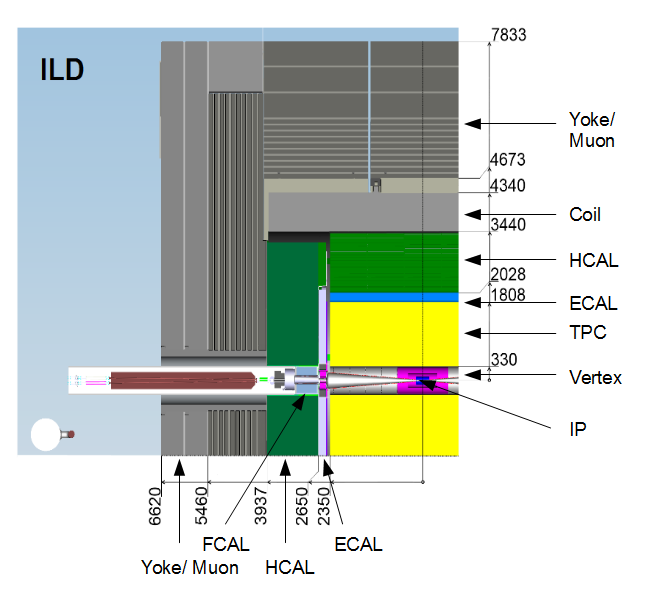
\includegraphics[width=.45\textwidth]{plots/ILD2}
\qquad
\caption{\label{fig:ILD} Longitudinal cross section of top quadrant of the ILD detector concept, taken from \cite{Behnke:2007gj}. From interaction point (IP) outwards, there is a tracking system compromising a large time projection chamber (TPC) augmented with silicon tungsten layer, highly granular electromagnetic calorimeters (ECAL) and hadronic calorimeters (HCAL), muon chambers, forward calorimeters (FCAL), magnetic coils and iron yokes. Numbers are in units of mm.
}
\end{figure}

The efficient tau lepton decay mode separation relies on the ability to reconstruct decay particles. Reconstruction of individual particles relies on highly granular detectors and sophisticated pattern recognition software to exploit the information. The PandoraPFA \cite{Marshall:2015rfa} particle flow software implements a sophisticated multi-algorithm particle reconstruction. It has been used in physics simulation  and detector optimisation studies for future linear collider, such as the Compact Linear Collider\cite{Linssen:2012hp} or the International Linear Collider\cite{Brau:2007zza}. Fitted helices of the hits in the tracking systems are projected to the front of the ECAL to associate calorimeter hits, and to form charged particles. Photons are reconstructed from calorimeter hits in the ECAL. A match is required between the photon clusters and the expected electromagnetic shower profiles. Neutral hadrons are reconstructed from calorimeter hits in the ECAL and the HCAL. The output of the PandoraPFA is a list of reconstructed particles, ``Particle Flow Objects'' (PFOs), which contains energy, momentum, position and particle id information.

%requires excellent spatial detector resolution, which is possibly  high granular calorimeters. 



%The particle flow approach to calorimetry relies on the ability to reconstruct individual particles. Consequently, this approach provides the possibility for highly efficient tau decay mode classification. 


The ability to accurately separate tau decay modes relies strongly on the efficient  photon reconstruction. Calorimeter hits in the ECal are clustered and carefully isolated from nearby charged particles. These photon candidates are compared with expected electromagnetic shower profiles. A likelihood based classifier is used to determine the photon id. Separate algorithms split merged photons and combine small photon fragments to main photons. Photon reconstruction in PandoraPFA is described in \cite{Xu:2016rcz}.

%The difficulty of the \PGt decay mode separation is to correctly reconstruct photons in the final states. Two main features of the reconstruction software, PandoraPFA \cite{Marshall:2015rfa}, help to separate the final states. Firstly, the iterative track cluster association algorithms connecting reconstructed tracks to the cluster showers in the calorimeters, providing a good identification of the charged particles and leave a cleaner environment for the neutral particles. Secondly, a transverse calorimeter shower profile based photon reconstruction algorithm carefully identifies and separates nearby photons, using a likelihood photon identification algorithm. Along side with other reconstruction algorithms in the PandoraPFA software, charged particles and photons are well reconstructed and used as inputs for \PGt decay mode separation.

This paper is organised in the following way: event simulation and reconstruction, selected decay modes, pre-selection, discriminating varibles, \decayRhoShort and\decayAiPhotonShort resonance, multivariate analysis, results and the ECAL optimisation study.

\section{Simulation and Reconstruction}
\label{section:MC}


Monte Carlo (MC) samples were generated with the generator software WHIZARD 1.95 \cite{whizard}.  PYTHIA 6.4 \cite{Sjostrand:1995iq},  tuned to the LEP results \cite{}, was used for the hadronisation. TAUOLA \cite{Jadach:1993hs} was used to describe the tau lepton decays, including the effect of the spin correlation between decay products. Events were simulated with software MOKKA \cite{MoradeFreitas:2002kj}, based on the GEANT 4 package  \cite{Agostinelli:2002hh}, with the ILD detector geometry description. Events reconstruction were performed using ilcsoft version v01-17-07 and PandoraPFA version v02-02-00, in the MARLIN software framework\cite{Gaede:2006pj}. Two million \eeToTauTau MC events were generated, for each ECal square cell size, and for each \rootS. In total, 48 million simulated events were generated. To maximise the impact of the ECAL design on the performance of the tau decay classification, the initial state radiation (ISR) and the beam induced background were not simulated, as these effects degrade the performance by the same amount irrespective of the ECAL design. 


\section{Selected decay modes}

Tau lepton decays into a numerous number of final states. To study the major effect of the tau lepton decays, decay modes with branching ratio above 1\% were chosen to study. This resulted in seven tau lepton decay modes considered, shown in table~\ref{tab:decay_mode}, which 92.58\,\% branching ratios of all tau lepton decays. 

\begin{table}[htbp]
\centering

\smallskip
\begin{tabular}{|l |l |c|}
\hline
  \textbf{Decay Mode} &  \textbf{Final State} & \textbf{Branching fraction / \%} \\
\hline
\PGtm$\to$\decayElectron   &  \decayElectron  & 17.83$\pm$0.04   \\
\PGtm$\to$\decayMuon  &	\decayMuon & 17.41$\pm$0.04  \\
\PGtm$\to$\decayPion  &   \decayPion	& 10.83$\pm$0.06   \\
  \PGtm$\to$\decayRho	& \decayRhoFinalState& 25.52$\pm$0.09 \\
  \PGtm$\to$\decayAiPhoton &\decayAiPhotonFinalState	& 9.30$\pm$0.11    \\
  \PGtm$\to$\decayAiPion  &	\decayAiPionFinalState    & 8.99$\pm$0.06  \\
  \PGtm$\to$\decayThreePionPhoton  &	\decayThreePionPhoton    & 2.70$\pm$0.08  \\

\hline
\end{tabular}
\caption{\label{tab:decay_mode} Branching fractions\cite{Agashe:2014kda} of the seven \PGtm decay modes and final states studied. \PGtp decays similarly to \PGtm.}
\end{table}


\section{Analysis}


\subsection{Event pre-selection}
\label{sec:presel}
Some events are very difficult or almost impossible to reconstruct correctly. This can happen if particles are in the forward beam pipe direction, where the forward calorimeters are not simulated due to computational limitations, or if particles carry too little energies to be significant than noises. Photons that converted into electron pairs in the tracking systems are reconstructed as an electron pair, which will alter the event topology and decrease the classification efficiencies. Also for the ILD detector model concept, the gap region between barrel part of the calorimeter and the end cap part causes a significant drop in the particle reconstruction efficiency. These effects do not vary with change of the ECAL square cell sizes in the later optimisation study. Therefore, unreconstructable events are discarded from the subsequent analysis. The selection efficiency of each cut is presented in table~\ref{tab:preselection}, using nominal ILD detector model and \rootS = 100\,GeV.


\begin{table}[htbp]
\centering

\smallskip
\small
\begin{tabular}{| l |p{25mm} | p{25mm} | p{35mm} |}
\hline
  Selection Efficiency in \%  & No \photonToee & No \photonToee and $E_{vis}>5GeV$ & No \photonToee, $E_{vis}>5GeV$, and decay in barrel or end cap \\
\hline

\textbf{\decayElectronShort}& 100.0 & 84.7& 66.2\\
\textbf{\decayMuonShort}&100.0& 85.2&66.7\\
\textbf{\decayPionShort}&100.0& 88.3&60.9\\
\textbf{\decayRhoShort}&77.1&76.9&61.9\\
\textbf{\decayAiPhotonShort}&61.3&61.2&50.5\\
\textbf{\decayAiPionShort}&100.0&100.0&78.0\\
\textbf{\decayThreePionPhotonShort}&77.0&77.0&61.8\\

\hline
\end{tabular}
\caption{\label{tab:preselection} Pre-selection efficiencies for seven tau decay modes, \decayElectron, \decayMuon, \decayPion, \decayRho, \decayAiPhoton, \decayAiPion, and \decayThreePionPhoton,  using nominal CLIC\_ILD detector model with \rootS = 100 \,GeV.}
\end{table}

An low visible energy event is discarded if the total energy of the tau lepton visible decay products is below 5\,GeV. Requirement of the tau decay in the barrel or the end cap part of the calorimeter is defined as the polar angle of the tau is $ 17.2\degree < |\theta_{Z}| < 34.4\degree$ or $ 45.8\degree < |\theta_{Z}| < 90\degree$.


%Events are discarded if simulated photons convert to electron pairs before reaching the calorimeters. Converted photons would not be reconstructed as photons, and events with converted photons would decrease the classification efficiency. That degradation would not be due to the calorimeter design.

%Events are also discarded if total energy of the tau lepton visible decay products is less than 5\,GeV. This ensures the decay products properly reconstructed.

%Events are further discarded if tau leptons are not within the barrel and end cap calorimeter regions. The polar angle for the end cap region is defined $ 17.2\degree < |\theta_{Z}| < 34.4\degree$. The polar angle for the barrel region is defined $ 45.8\degree < |\theta_{Z}| < 90\degree$. The forward-most part of the detector, close to the beam pipe, is not simulated due to technical reasons. The particle reconstruction was not optimised for the gap region between the barrel and the end cap region for the CLIC\_ILD detector. Therefore by confining to the barrel and the end cap region only, a consistent high particle reconstruction efficiency is ensured.




%The chosen final states can be classified into three categories: leptonic decays, one-prong with photons and three-prong with photons. 

\subsection{Select single tau decay}

For convenience, \eeToTauTau were used. Each of the taus was examined in turn. To select single tau decay, the scalar  dot product between the thrust axis and the momentum vector is used to separate particles into one of the two collections. Thrust axis is the normal vector, $\hat{n}$, that maximises, $T = max_{\hat{n}} \frac {\Sigma_{i} \left| p_i . \hat{n} \right|}{\Sigma_{i} \left| p_i \right|}$, where $p_i$ is the momentum vector of the $i^{th}$ particle.


\subsection{Discriminating variables}



% A selected few most important varibles are described in details.


Having pre-selected samples, a set of discriminating variables was carefully developed to be used in the later multivariate analysis (MVA). These variables allow the multivariate classifier achieves a highly efficient tau decay mode classification. Different variables have discriminative powers against different final states. For convenience, variables are presented sequentially, although they participate the MVA simultaneously.

To differentiate 1-prong final states from 3-prong final states, number of tracks, shown in figure~\ref{fig:nCharge}, provides excellent separation power. Selection efficiencies are over 95\% for the 1-prong final states, and over 90\% for the 3-prong final states. For the 1-prong final states, they are further separated based on the number of photons reconstructed. Clear distinction between \decayPion, \decayRho and \decayAiPhoton decays mode can be seen in figure~\ref{fig:nPhoton}, where the overlap between any two decay modes is below 15\%. The two leptonic decay modes, \decayMuon and \decayElectron, have very different event topologies to other decay modes. For the \decayMuon decay mode, only muons deposit energies in the muon chamber. For the \decayElectron decay mode, electrons shower in the ECAL can be modelled by electromagnetic shower profiles. This information is used to distinguish a electron from a charged pion, including comparison of the observed and the expected electromagnetic shower profile, the matching between inner detector tracks and calorimeter clusters, and the fraction of calorimeter hits registered as minimum ionised particles.





\begin{figure}[!tbp]
\centering % \begin{center}/\end{center} takes some additional vertical space

%\subfigure[Figure A]{\label{fig:a}\includegraphics[width=60mm]{example-image-a}}
\begin{subfigure}[b]{0.45\textwidth}
 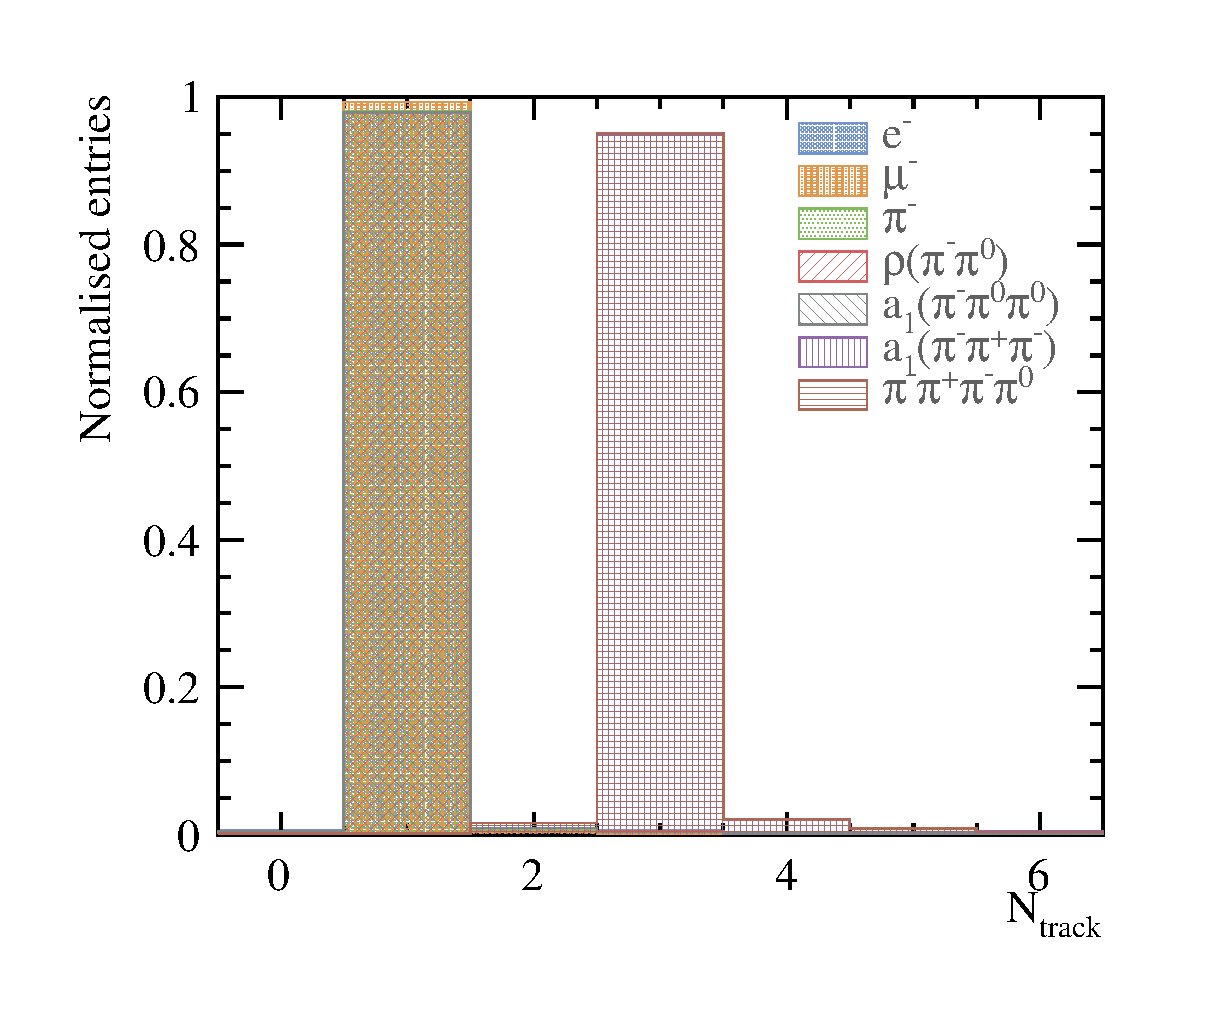
\includegraphics[width=\textwidth]{plots/var2/nCharge_100GeV_improved} 
  \caption{}
  \label{fig:nCharge}
\end{subfigure}
\begin{subfigure}[b]{0.45\textwidth}
 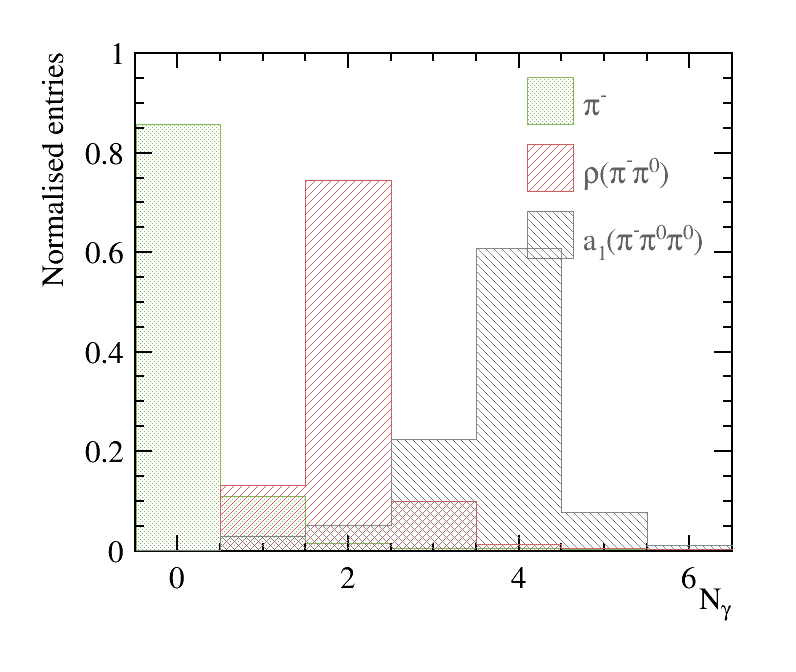
\includegraphics[width=\textwidth]{plots/var2/nPhoton_100GeV_improved} 
  \caption{}
  \label{fig:nPhoton}
\end{subfigure}

\begin{subfigure}[b]{0.45\textwidth}
 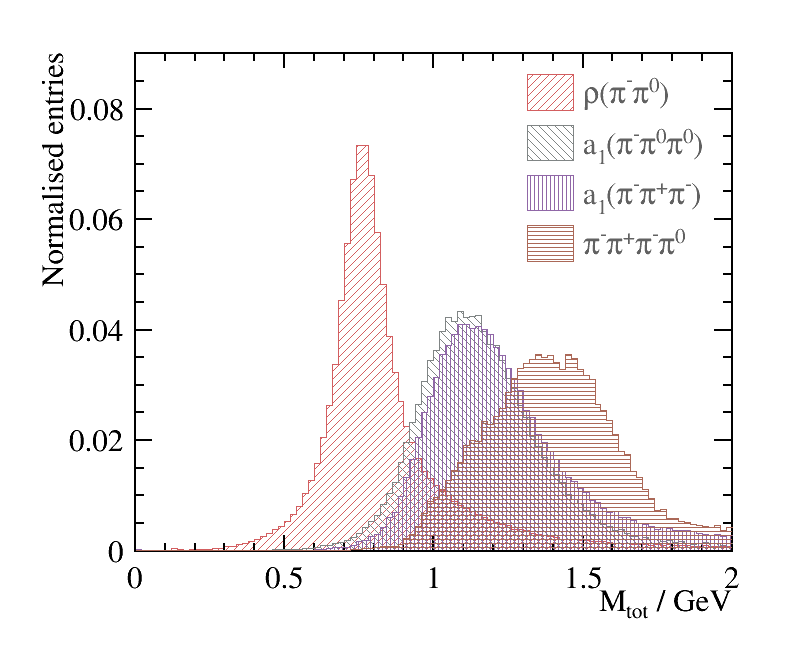
\includegraphics[width=\textwidth]{plots/var2/mVis_100GeV_improved_zoom}
  \caption{}
  \label{fig:mVis}
\end{subfigure}
\begin{subfigure}[b]{0.45\textwidth}
 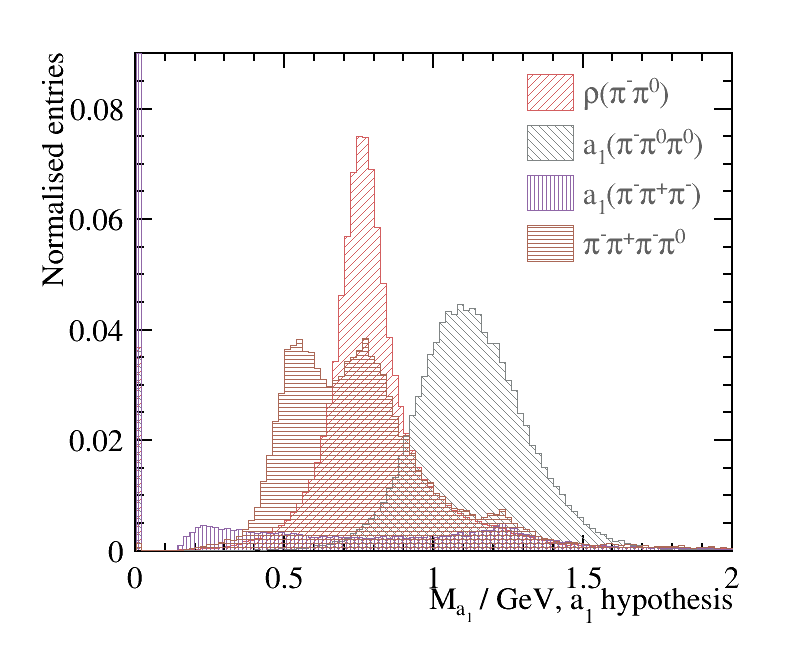
\includegraphics[width=\textwidth]{plots/var2/mA1A1Fit_100GeV_improved_zoom}
  \caption{}
  \label{fig:mA1}
\end{subfigure}

\caption{Normalised distribution for discriminative variables for seven tau decay modes, \decayElectron, \decayMuon, \decayPion, \decayRho, \decayAiPhoton, \decayAiPion, and \decayThreePionPhoton,  with \rootS = 100\,GeV for nominal ILD detector model. Figure~\ref{fig:nCharge} is the number of tracks. Figure~\ref{fig:mVis} is the invariant mass of visible PFOs.  Figure~\ref{fig:nPhoton} is the number of photons. Figure~\ref{fig:mA1} is the invariant mass of \decayAiPhotonShort, calculated with \AiPhotonDecay resonance reconstruction. 
}
\label{fig:var} 
\end{figure}

\subsection{Reconstruction of \texorpdfstring{\PaDoP{1260}}{a1} and \texorpdfstring{\PGrP{770}}{$\rho$}  resonances}

Varibles described above separate 1-prong final states from 3-prong final states, and separate different 1-prong final states. Figure~\ref{fig:mVis} shows the differences in the total invariant mass. However, there is an overlap between the mass distribution for different decay modes. To further enhance the separation of the \decayAiPhoton and \decayRho, the \PaDoP{1260} and \PGrP{770} resonances are reconstructed by considering all possible combination of reconstructed photon candidates. For example, the \AiPhotonDecay decay produces four photons. If two photons are very close together, they can be merged in the reconstruction. Alternatively, if some of the energy deposition from the \PGpm appears as fragments, additional photon photons can be reconstructed. To enhance the resonance reconstruction, \decayAiPhoton decay is reconstructed by minimising $\chi_{\Pa}^{2}$, defined as
\begin{equation}
\label{eq:a1}
\chi_{\Pa}^{2} = {\left(\frac{m^*_{\Pa} -  m_{\Pa}}{\sigma_{\Pa}}\right)}^{2} + {\left(\frac{{m^*_{\PGpz,1}} -  m_{\PGpz}}{\sigma_{\PGpz,1}}\right)}^{2} + {\left(\frac{{m^*_{\PGpz,2}} -  m_{\PGpz}}{\sigma_{\PGpz,2}}\right)}^{2}  \,,
\end{equation}
where $m^*_{\PGpz,1}$ and $m^*_{\PGpz,2}$  are the invariant masses of two photons combinations, $\sigma_{\Pa}$ and $\sigma_{\PGpz}$ are the half width of the invariant mass distribution of reconstructed \Pa and \PGpz using the truth information, and $m_{\Pa}$ and $m_{\PGp}$ are the masses of \Pa and \PGpz, taken from \cite{Agashe:2014kda}. This improves the invariant mass of the \PaDoP{1260} resonance. Shown in figure~\ref{fig:mA1}, only the \decayAiPhoton decay mode has a peak structure at the \PaDoP{1260} resonance, and there is a little overlap between \decayAiPhoton decay mode and other decay modes comparing to the distribution in the figure~\ref{fig:mVis}.

The \RhoDecay decay has the similar reconstruction issue, and is enhanced with a similar $\chi^{2}$ minimisation. It results in similar improvement in \PGrP{770} resonance reconstruction and better separation between  the \decayRho decay mode and other decay modes.


%Additional variables are calculated using the calorimeter information, the comparison with the electromagnetic shower profile, the matching between the track and the cluster, the energy and invariant masses for different types of particles. Extra variables regarding to the electromagnetic shower profile are used to distinguish electrons from charged pions.

%, listed in Table XX. Note that XX variables were specialised in separating a electron from a pion. XX variables were made to test the hypothesis of XX particles. The rho hypothesis is to find the best rho decay candidates by minimising chi squared according to $aa$, where X is all possible charge pions, Y is all possible 2 photons. The formula will reduce accordingly if there is 1 photon. Similarly, the a1 decaying to 1 pion 4 photon hypothesis is done in a same fashion with Chi squared function XX, , where X is all possible charge pions, Y is all possible 2 photons. The formula will reduce accordingly if there are 2 or 3 photons.

%The variables of energy ratios instead of the raw energies were calculated to make the MVA process more generic across different c.o.m. energies.


\subsection{Multivariate analysis}



A set of 29 discriminating variables was used to classify tau decays into one the following decay modes: \decayElectron, \decayMuon, \decayPion, \decayRho, \decayAiPhoton, \decayAiPion, and \decayThreePionPhoton. The variables fall into 5 distinctive categories. Energy variables include:
\begin{itemize}
\item  Total energy deposited in ECal and HCal, divided by the total energy of charged PFOs,  
\item  Total energy deposited in ECal and HCal, divided by the total energy of all PFOs,  
\item  Invariant mass of total PFOs in GeV,   
\item  Total energy of all PFOs, divided by the energy of the \PGtm, 
\item  Total energy of charged PFOs, divided by the energy of \PGtm,    
\item  Total energy of muons, divided by the energy of \PGtm,    
\item  Total energy of electrons, divided by the energy of \PGtm,
\item  Total energy of photons, divided by the energy of \PGtm,  
\item  Total energy of charged pions, divided by the energy of \PGtm    
\end{itemize}
where the energy of the \PGt is taken to be the same as the energy of \Pepm beam, which is half of the \rootS energy. 

Invariant mass variables include:
\begin{itemize}
 
\item Invariant mass of charged PFOs in GeV,   
\item Invariant mass of neutral PFOs in GeV,   
\item Invariant mass of photons in GeV,  
\item Invariant mass of charged pions in GeV.   
\end{itemize}

Number of PFOs variables include:
\begin{itemize}
\item  Number of charged PFOs,    
\item  Number of muons,
\item  Number of electrons,
\item  Number of photons,
\item  Number of charged pions.
\end{itemize}

Variables to distinguish electrons from charged pions include:
\begin{itemize}
\item  Average energy deposited in a calorimeter cell in GeV,
\item  Average transverse shower width, for all clusters in the ECal,
\item  Average longitudinal shower start layer for all clusters in the ECal,
\item  Average discrepancy in longitudinal electromagnetic shower between the observed and the expected profile, for all clusters in the ECal,
\item Average fraction of calorimeter hits registered as minimum ionised particles, all clusters in the ECal,
\item  Average ratio between  energy and momentum, for all clusters in the ECal,
\end{itemize}

The \PaDoP{1260} and \PGrP{770} resonances reconstruction variables include:
\begin{itemize}
\item  Best reconstructed invariant mass of  \PaDoP{1260}, for \PaDoP{\PGpm\PGpz\PGpz} resonance reconstruction,

\item  Best reconstructed invariant mass of \PGpz, for \PaDoP{\PGpm\PGpz\PGpz} resonance reconstruction,
\item  Second best reconstructed invariant mass of \PGpz, for \PaDoP{\PGpm\PGpz\PGpz} resonance reconstruction,


\item  Best reconstructed invariant mass of \PGrP{770}, for \PGrP{\PGpm\PGpz} resonance reconstruction,
\item  Best reconstructed invariant mass of \PGpz, for \PGrP{\PGpm\PGpz} resonance reconstruction.
\end{itemize}


For the multivariate analysis, the multiclass of the TMVA package \cite{Therhaag:2009dp} was used to perform a multiclass classification, which trains the seven final states simultaneously. The multiclass class is an extension of the standard two-class signal-background classifier. For each final state, the multiclass classifier will train the final state as the signal against all other final states as the background. This process is repeated for each final state. The classifier output for a single event is a normalised response for each final state, where the sum is one. The response of each final state of an event can be treated as the likelihood. The event is classified into a particular final state if the final state has the highest classifier output response. The advantage of using the multiclass is that the correlation between different final states are accounted for and the classifier output are correctly adjusted for multiple final states, hence one event can only be classified into one final state. The issue with the multiclass is that discriminative variables for each decay mode need enter the training stage, resulting in a large number of variables. 

Half of the events, randomly selected, were used in the training process and the other half were used for testing. The TMVA multiclass classifier is a boosted decision tree with gradient boosting (BDTG), as it was found to give for the best performance.  The MVA classifier is trained and optimised to give the best product of correction classification probabilities of all final states.

\section{Results}

Using the discriminating variables and trained the MVA classifier, the classification results of the MVA is shown in table~\ref{tab:sel_example}, for seven tau decay modes of  using  the nominal ILD detector model, for \rootS = 100\,GeV. A perfect classification would only have diagonal terms in the table. 

%The reconstruction efficiencies for the seven final state of the tau decaying with c.o.m. energy of 100 \,GeV for the nominal CLIC\_ILD detector are shown in the 
%For the leptonic decays, the correct classification probabilities are above 99.5\%, aided by the tracking system, which offers precision position and momentum measurements.


\begin{table}[htbp]
\centering

\smallskip
\small
\begin{tabular}{| l | r | r | r | r | r | r | r |}
\hline
  \textbf{Reco $\downarrow$ True $\to$}  & \textbf{\decayElectronShort} & \textbf{\decayMuonShort} &\textbf{\decayPionShort} & \textbf{\decayRhoShort} &\textbf{\decayAiPhotonShort} &\textbf{\decayAiPionShort} &\textbf{\decayThreePionPhotonShort} \\
\hline

\textbf{\decayElectronShort}&\textbf{99.7}&-&0.9&0.6&0.4&-&-\\
\textbf{\decayMuonShort}&-&\textbf{99.5}&0.6&-&-&-&-\\
\textbf{\decayPionShort}&-&0.3&\textbf{94.0}&0.8&-&0.4&-\\
\textbf{\decayRhoShort}&-&-&3.4&\textbf{93.6}&9.5&0.6&2.3\\
\textbf{\decayAiPhotonShort}&-&-&-&4.5&\textbf{89.7}&-&0.6\\
\textbf{\decayAiPionShort}&-&-&0.9&-&-&\textbf{96.8}&6.4\\
\textbf{\decayThreePionPhotonShort}&-&-&-&0.3&-&2.0&\textbf{90.6}\\


\hline
\end{tabular}
\caption{\label{tab:sel_example} Classification probability in percentage for tau decay modes using the nominal ILD detector model , for \rootS = 100 \,GeV . Bold numbers show the correct classification probability. Numbers below 0.25\%, and \PGnGt are not shown in decay modes, for display purposes. Statistical uncertainties are less than 0.25\%.}
\end{table}

The correct classification probability reflects the difficulty to classify a final state. The \decayMuonShort and \decayElectronShort decay modes have 99.5\% and 99.8\% correct classification probabilities, as these two decay modes have very different topologies. For 1-prong final states, wrong classification mainly occur between the \decayPionShort, \decayRhoShort, and \decayAiPhotonShort decay modes, because if two photons are very close together, they can be merged and the information about the two photons are lost. For 3-prong final states, wrong classifications mainly occur between \decayAiPionShort, and \decayThreePionPhotonShort, for the similar reason that photons close together can be merged and the information is lost. A correct classification probability over 88.2\% for each tau decay mode is achieved, using the nominal ILD detector with \rootS = 100\,GeV. 

\section{Electromagnetic calorimeter optimisation}

To study of the impact of the ECal square cell sizes on the classification of tau decays, the above procedure was repeated for ECal square cell sizes at 3, 5, 7, 10, 15 and 20\,mm, at four  \rootS energy of 100, 200, 500, 1000\,GeV. Other ECAL dimensions were kept constant. Because the lepton reconstruction mostly rely on the tracking system, which was not varied in this study, only the  hadronic tau decays were investigated and compared between different ECAL square cell sizes.

\subsection{Impact of ECal square cell sizes}

\begin{figure}[!tbp]
\centering % \begin{center}/\end{center} takes some additional vertical space
\begin{subfigure}[b]{0.45\textwidth}
  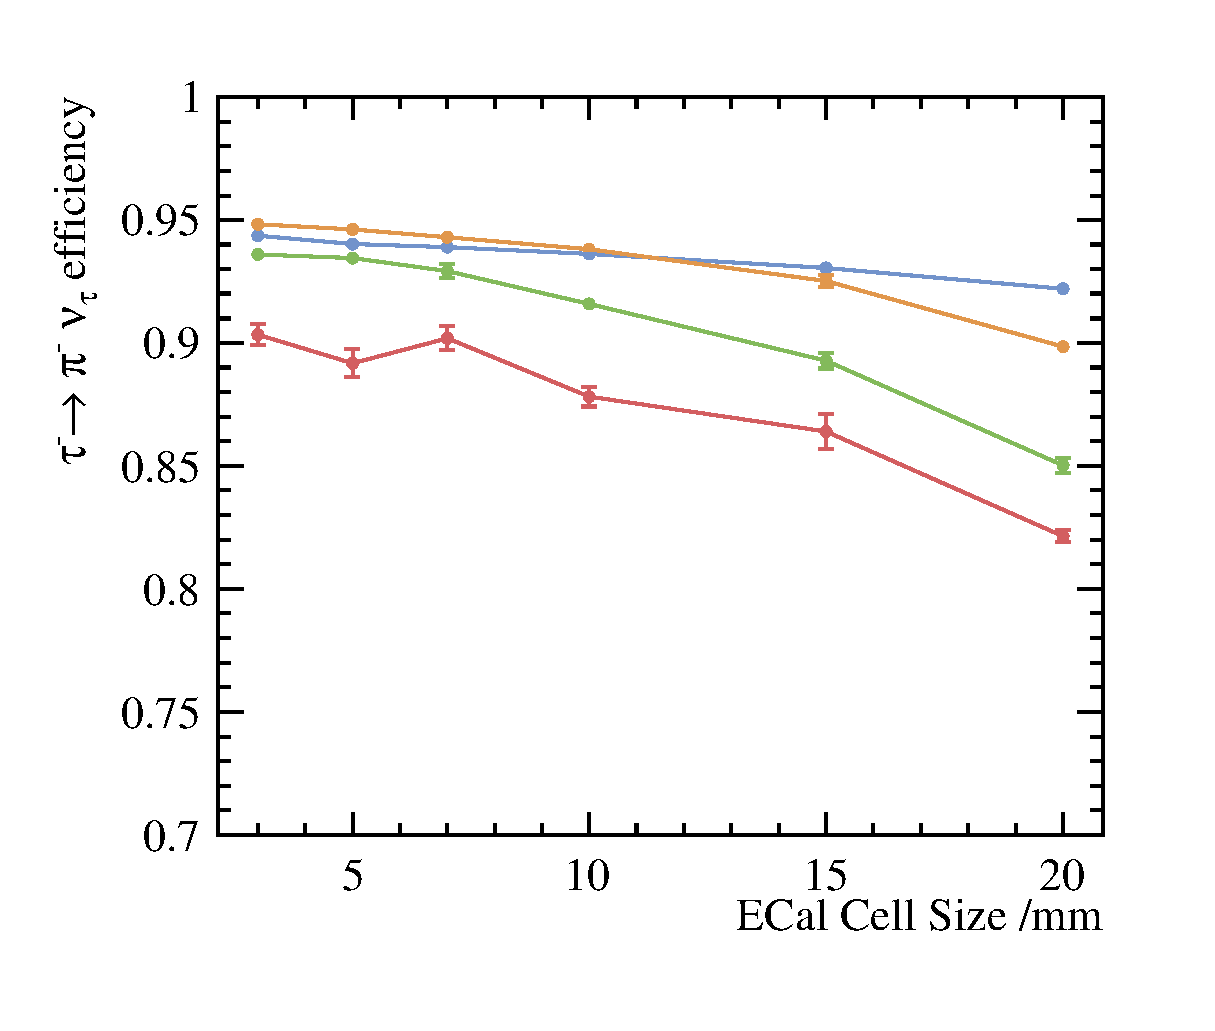
\includegraphics[width=\textwidth]{plots3/decayMode2}
  \caption{}
  \label{fig:decayMode2}
\end{subfigure}
\begin{subfigure}[b]{0.45\textwidth}
  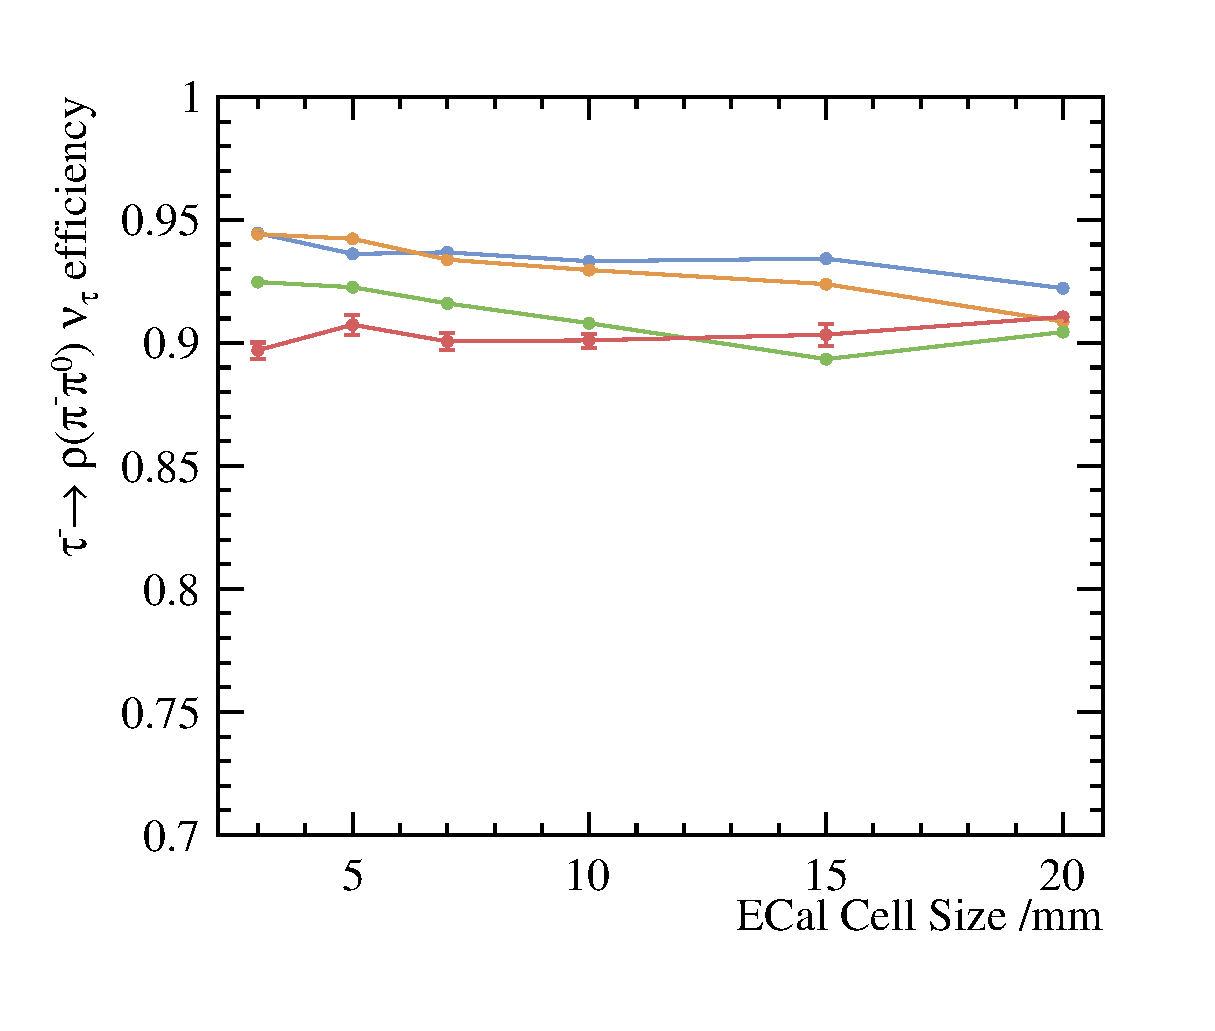
\includegraphics[width=\textwidth]{plots3/decayMode3}
  \caption{}
  \label{fig:decayMode3}
\end{subfigure}
\begin{subfigure}[b]{0.45\textwidth}
  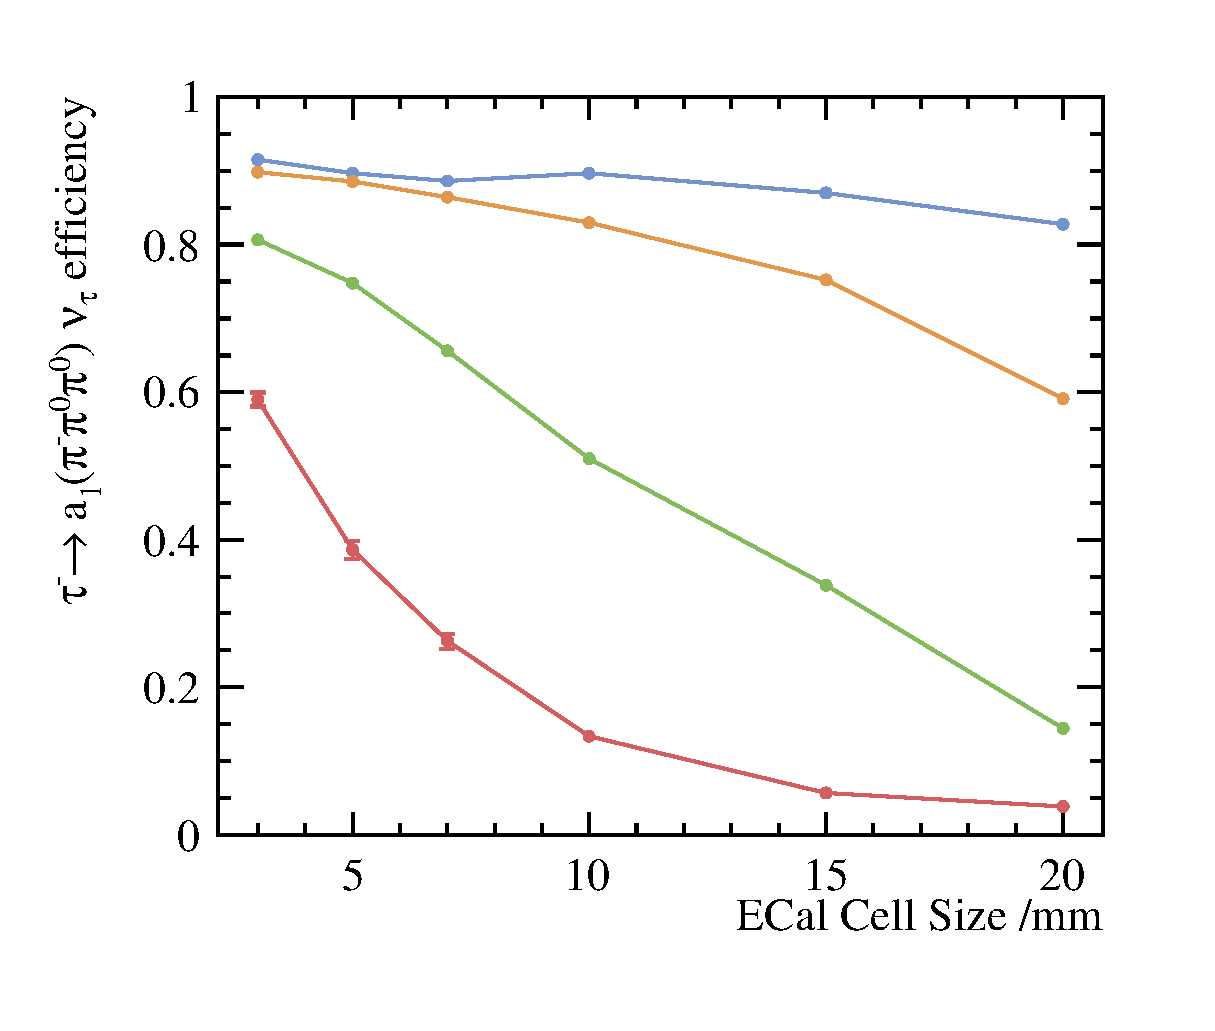
\includegraphics[width=\textwidth]{plots3/decayMode4}
  \caption{}
  \label{fig:decayMode4}
\end{subfigure}
\begin{subfigure}[b]{0.45\textwidth}
  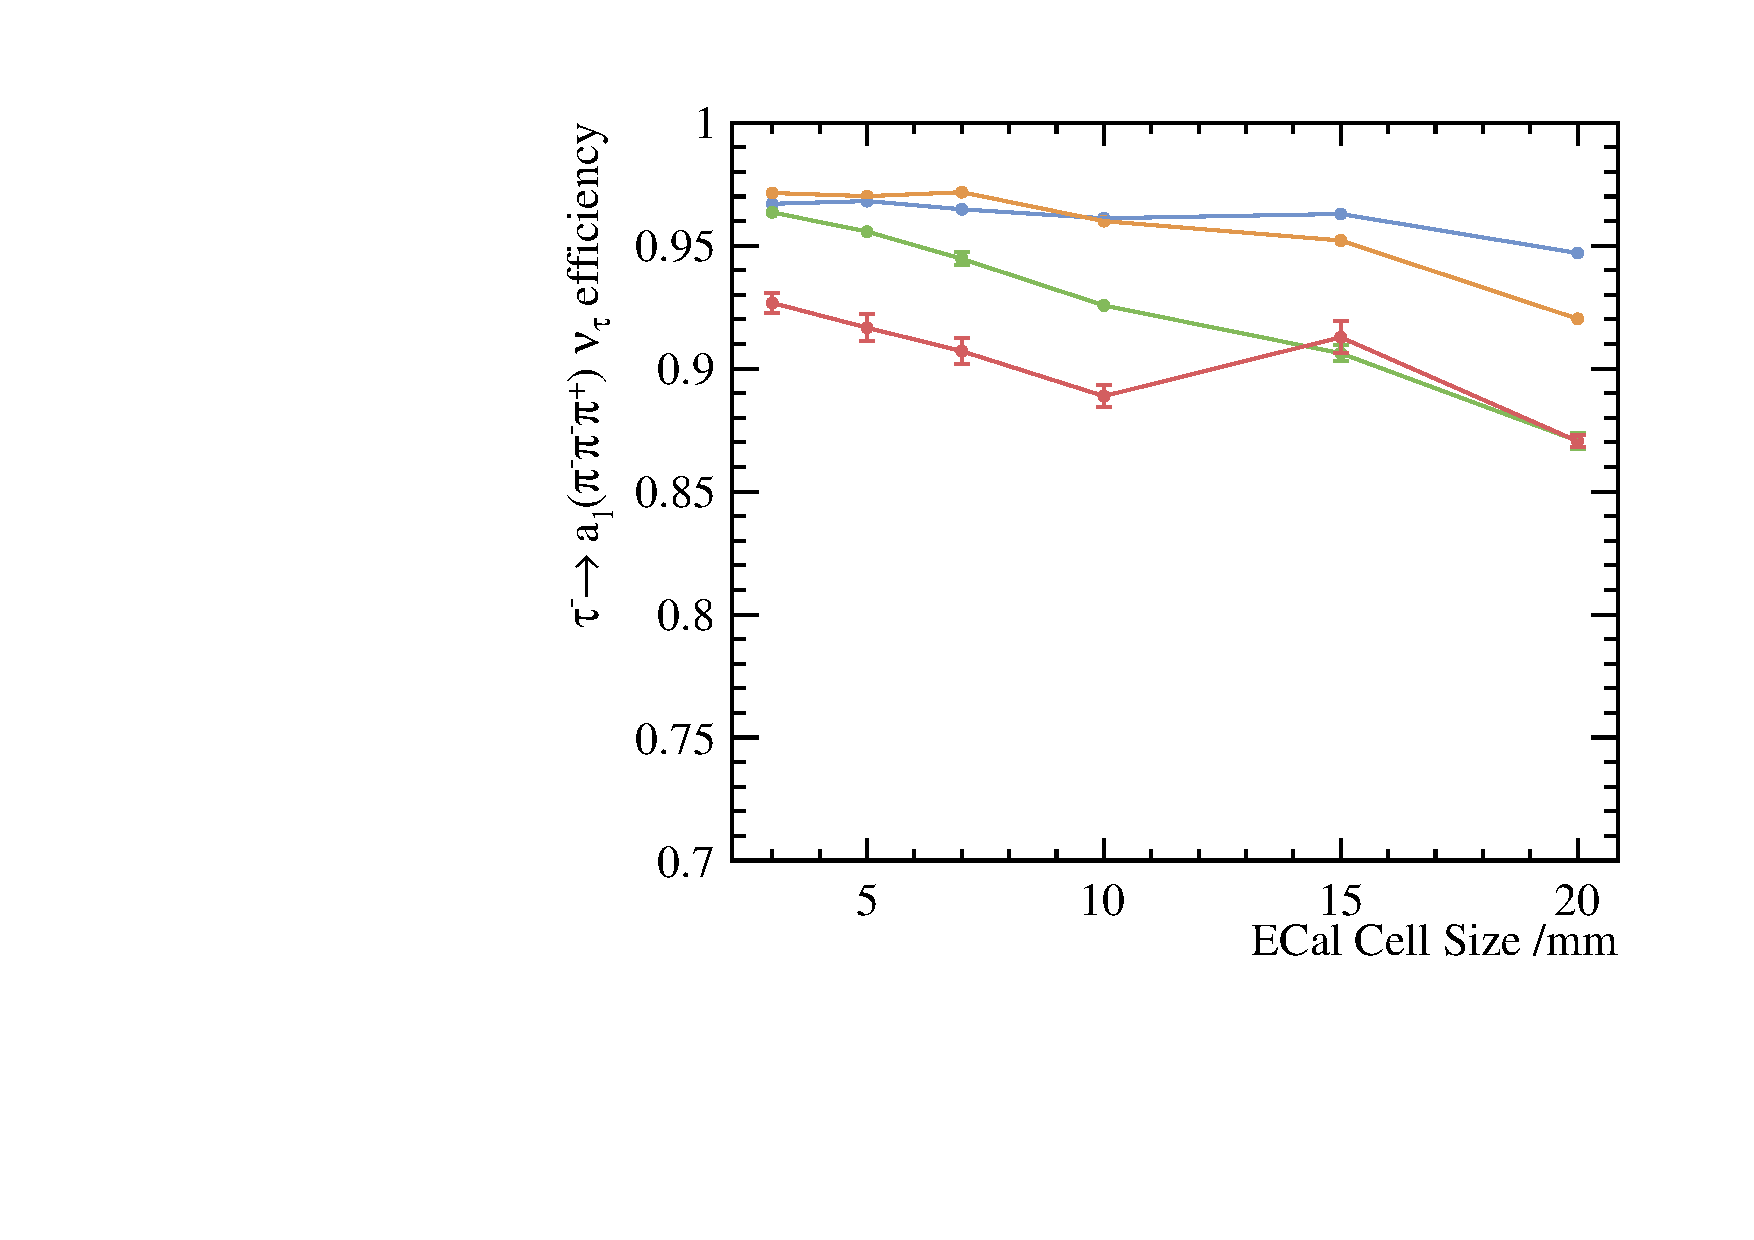
\includegraphics[width=\textwidth]{plots3/decayMode5}
  \caption{}
  \label{fig:decayMode5}
\end{subfigure}
\begin{subfigure}[b]{0.45\textwidth}
  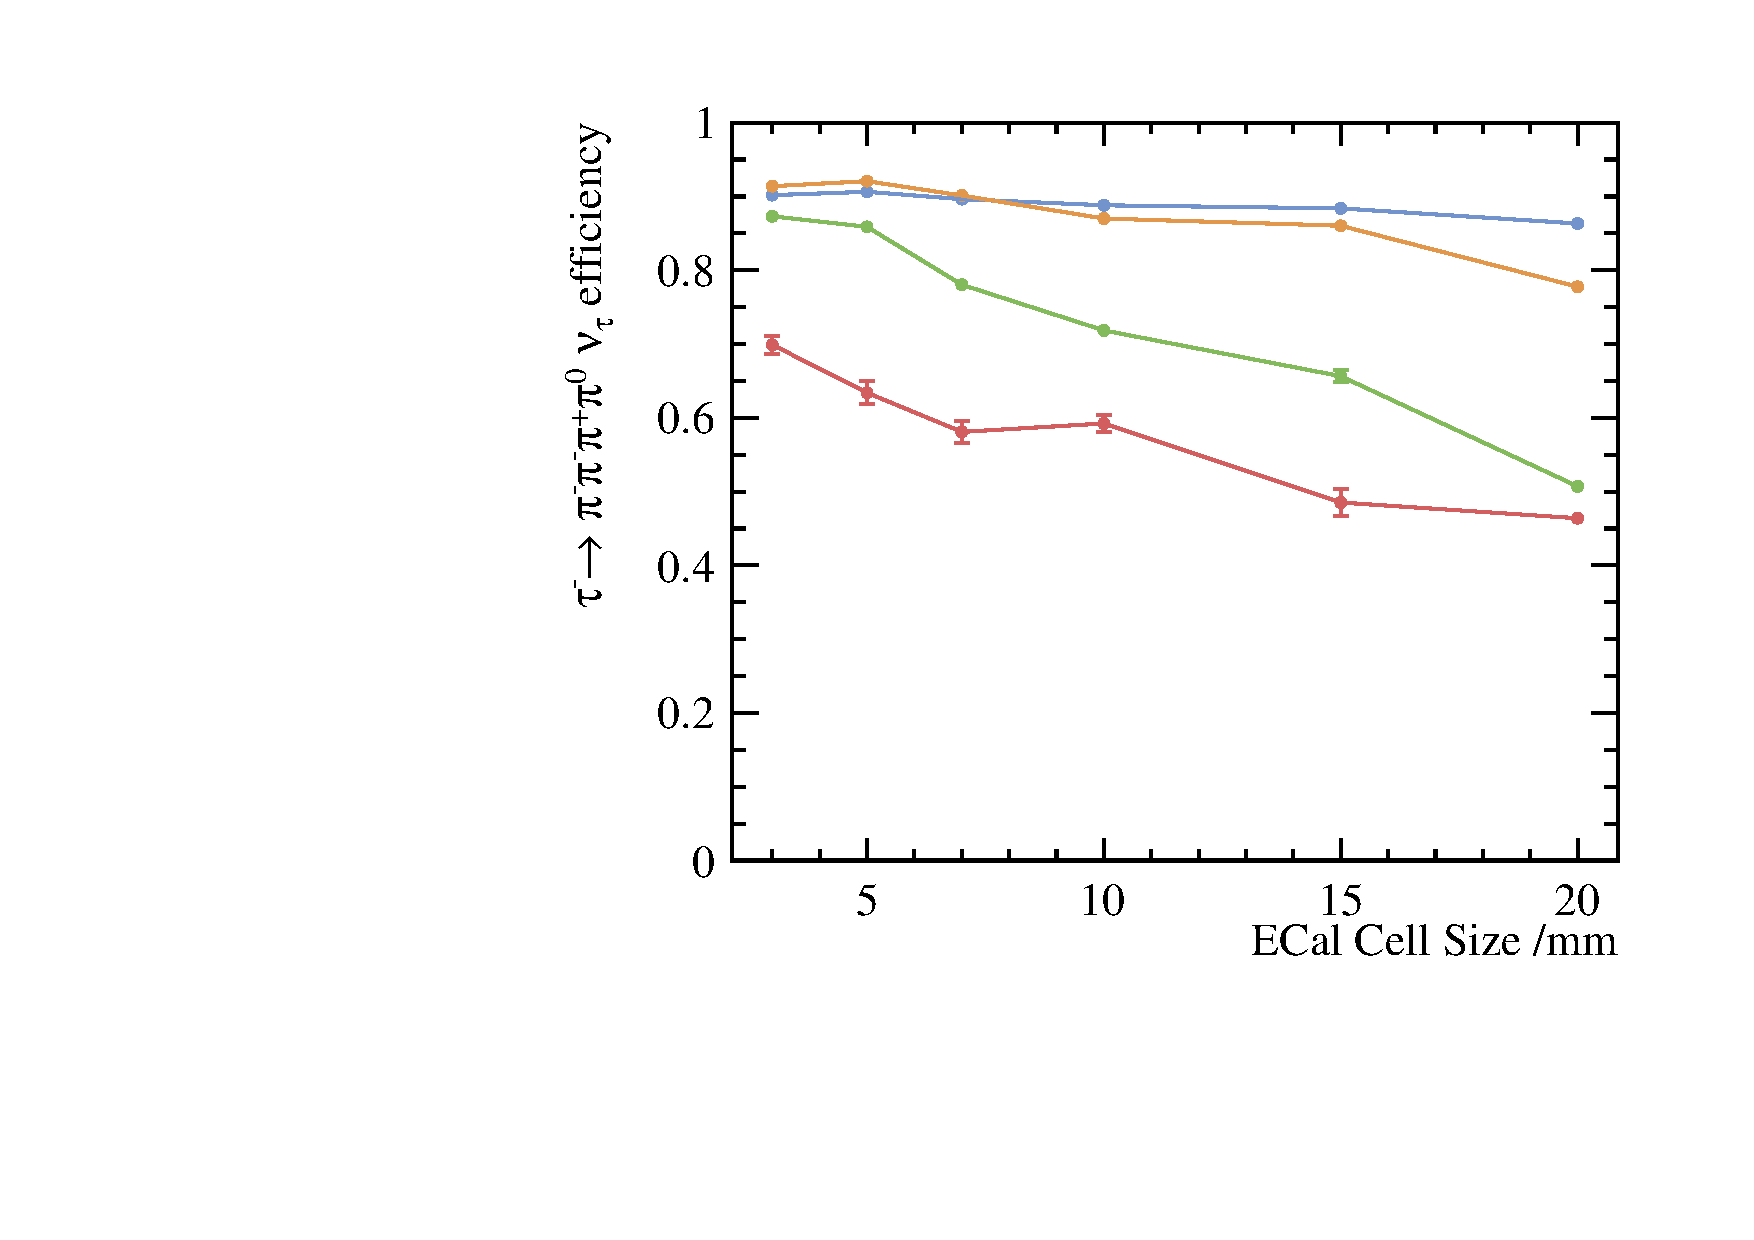
\includegraphics[width=\textwidth]{plots3/decayMode6}
  \caption{}
  \label{fig:decayMode6}
\end{subfigure}
\begin{subfigure}[b]{0.45\textwidth}
  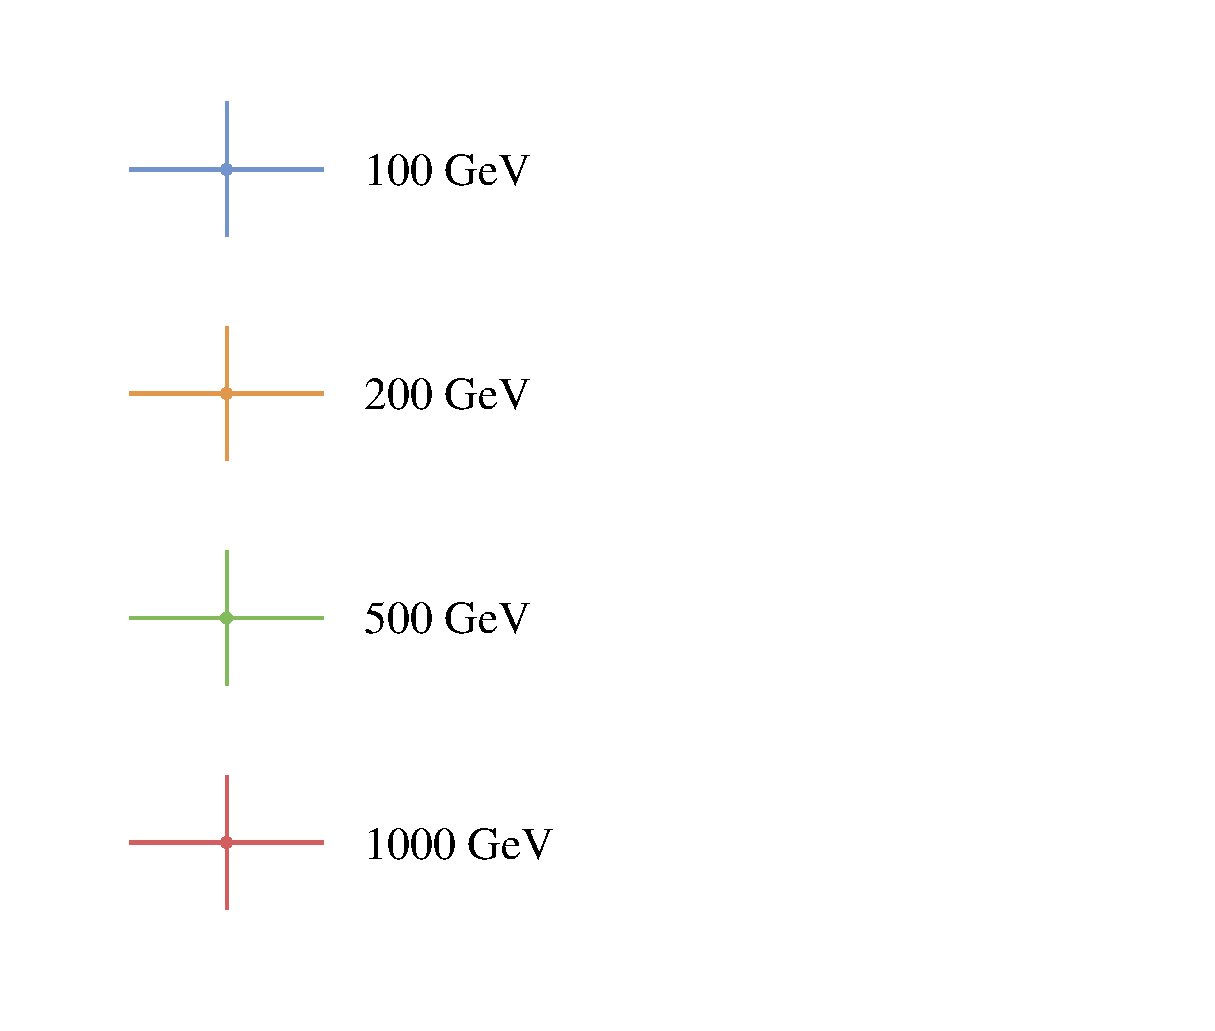
\includegraphics[width=\textwidth]{plots3/legend}
  %\caption{}
  %\label{fig:legend}
\end{subfigure}
\caption{\label{fig:pion_efficiency} The correct classification probabilities for hadronic tau decay final states  as a function of the ECal square cell sizes, using the nominal CLIC\_ILD detector model with \rootS = 100, 200, 500 and 1000\,GeV. Figure~\ref{fig:decayMode2}, ~\ref{fig:decayMode3}, ~\ref{fig:decayMode3}, ~\ref{fig:decayMode4}, ~\ref{fig:decayMode5} show the \decayPion, \decayRho,  \decayAiPhoton, \decayAiPion  and \decayThreePionPhoton  decay modes, respectively. Blue, orange, green and red lines represents  \rootS = 100, 200, 500 and 1000\,GeV respectively. Note that the the scale on the y axis are not the same, for display purposes.}
\end{figure}
%\qquad
%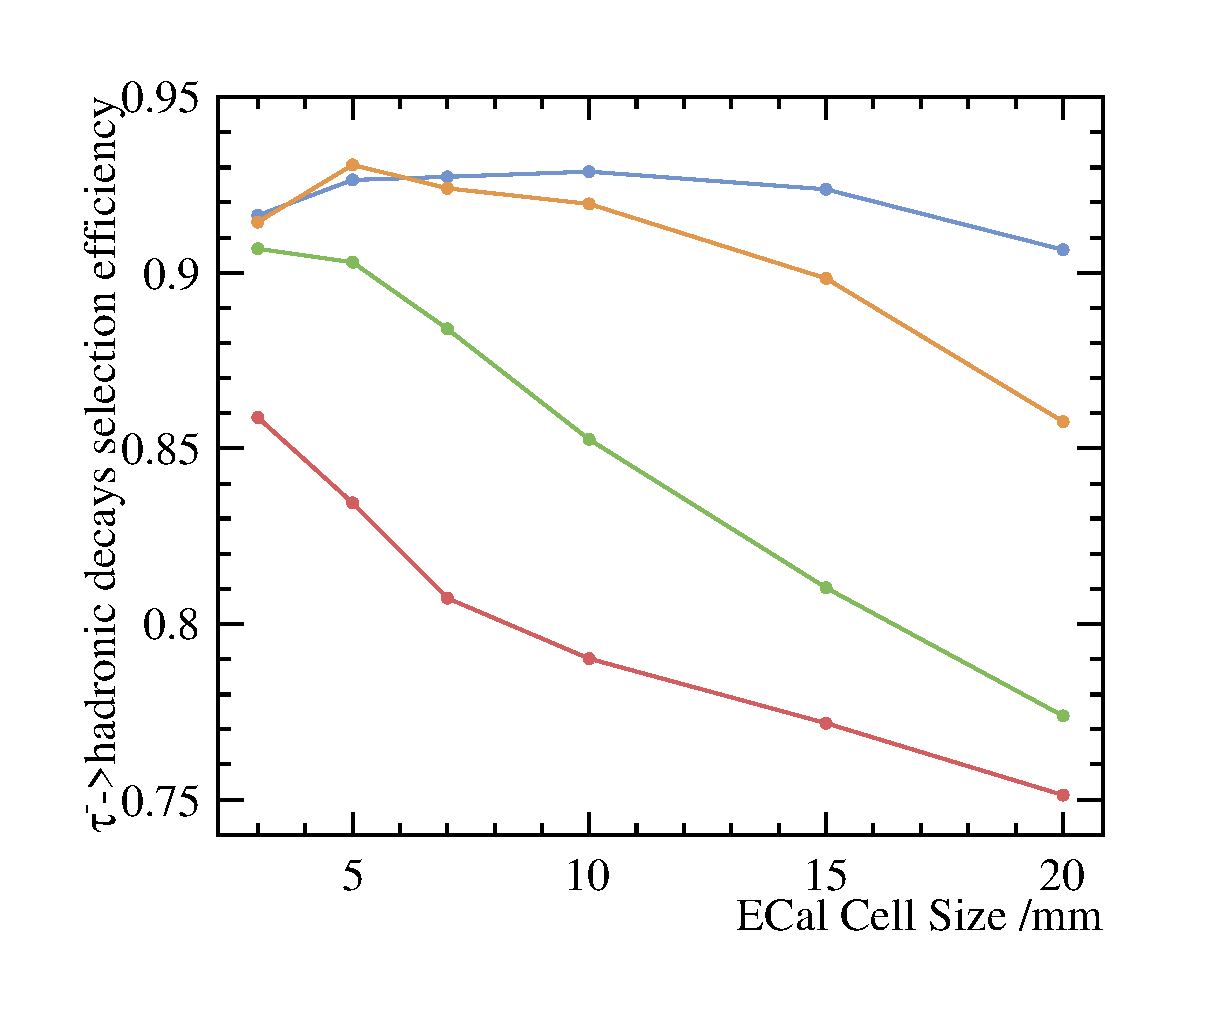
\includegraphics[width=.4\textwidth]{plots/hadEff}
% "\includegraphics" from the "graphicx" permits to crop (trim+clip)
% and rotate (angle) and image (and much more)


Figure~\ref{fig:pion_efficiency} shows correct classification probabilities for hadronic tau decay final states as a function of the ECal square cell sizes, using the nominal CLIC\_ILD detector model with \rootS = 100, 200, 500 and 1000\,GeV. Overall, the correct classification probabilities for hadronic tau decays decrease with increasing \rootS and increasing ECAL cell sizes. At a higher \rootS, decay products are closer together in the detector, and therefore it is more difficult to reconstruct individual decay product. A larger ECAL cell sizes offers a lower spatial resolutions. The reconstruction of two photons close together is more difficult. If photons are merged in the reconstruction, classification between different decay modes is more challenging and the correct classification probability is lower.


For the \decayRho decay mode, shown in figure~\ref{fig:decayMode3}, the correct classification probabilities for \rootS = 500\,GeV rises for ECal square cell sizes from 15 to 20\,mm, and for  \rootS = 1000\,GeV from 7, to 20\,mm. This is due to the optimisation of the MVA favours the overall correct classification rate, which can be seen in the sharp drop in correct classification probabilities for the \decayAiPhoton decay mode for the same \rootS and the same energy, shown in figure~\ref{fig:decayMode4}. 

TODO:
For \rootS = 100 and 200\,GeV, the correct classification probabilities for the 5\,mm ECal cell size is better than that of the 3\,mm. This is most noticeably shown in figure~\ref{fig:decayMode4}. One possible explanation is that PandoraPFA has been optimised for the nominal ILD detector with the 5\,mm ECal cell size, which shares the same ECal structure with the nominal CLIC\_ILD detector.




\subsection{Tau hadronic decay correct classification probability}

\begin{figure}[htbp]
\centering % \begin{center}/\end{center} takes some additional vertical space
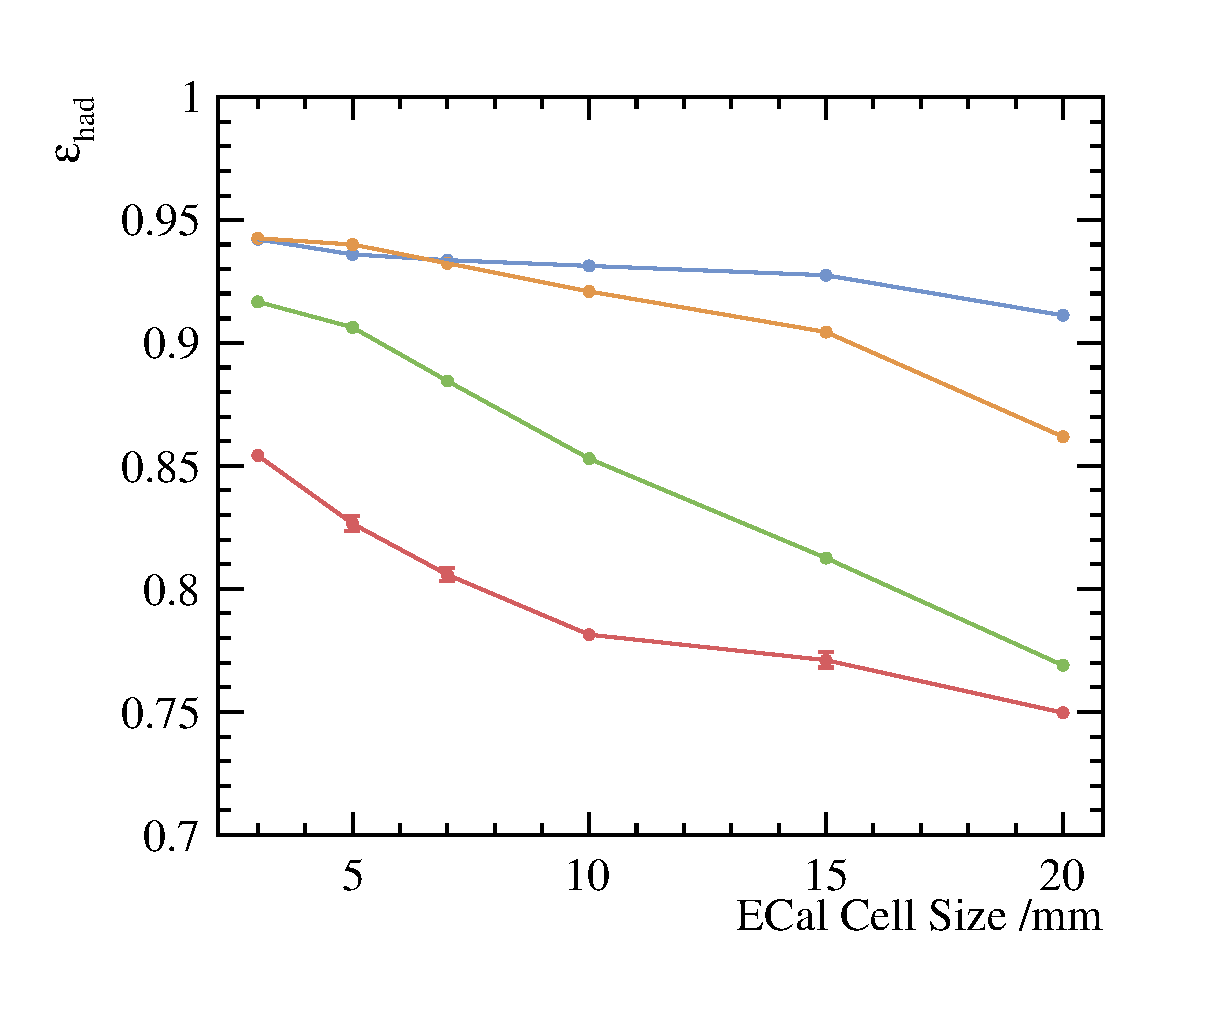
\includegraphics[width=.45\textwidth]{plots3/hadronicEff}
% "\includegraphics" from the "graphicx" permits to crop (trim+clip)
% and rotate (angle) and image (and much more)
\caption{\label{fig:hadronic_efficiency} The tau lepton hadronic decay correct classification probability, $\varepsilon_{had}$, as a function of the ECal square cell size for different \rootS. Blue, orange, green and red lines represent \rootS = 100, 200, 500 and 1000\,GeV, respectively.}
\end{figure}

Overall classification performance across all decay modes can be compared by constructing a single parameter function, which is a weighted average of the correct classification probability for each decay modes. This single parameter allows the direct comparison between different ECal cell sizes, for different \rootS. The chosen single parameter function is the tau lepton hadronic decay correct classification probability, $\varepsilon_{had}$, defined as
\begin{equation}
\label{eq:had}
\varepsilon_{had} = \frac{\left(\Sigma_{i} {Br}_{i}\varepsilon_{i}\right)}{\Sigma_{i} {Br}_{i}}  \,,
\end{equation}
where $Br_{i}$ is the branching ratio of a hadronic decay mode after the generator level cut in section~\ref{sec:presel}. $\varepsilon_{i}$ is the correct classification probability for decay mode $i$. Figure~\ref{fig:hadronic_efficiency} shows  $\varepsilon_{had}$ as a function of the ECal square cell size for different \rootS. As expected  $\varepsilon_{had}$ decreases with increasing ECal square cell sizes, and increasing \rootS.




TODO:
//For \rootS = 100 and 200\,GeV, $\varepsilon_{had}$ for the 5\,mm ECal square cell size is better than that of the 3\,mm. This is possibly due the optimisation of the software for the nominal ILD 5\,mm square cell size.


CONCLUSION MAY CHANGE
For the ILC 500\,GeV and the CLIC 350\,GeV  scenarios, larger ECAL square cell sizes up to 15\,mm have a small impact on $\varepsilon_{had}$. The decrease in $\varepsilon_{had}$  from 3\,mm to 15\,mm ECAL cell for \rootS = 100 and 200\,GeV is below 4\%.  For the ILC 1\,TeV and the CLIC 1.4\,TeV and 3\,TeV scenarios, an increase of 1\,mm in the ECAL square cell size leads a decrease of approximately 0.8\% in $\varepsilon_{had}$. To achieve a high $\varepsilon_{had}$, a small ECAL cell size is needed.


%ECal square cell size has a bigger impact on higher \rootS. For \rootS = 100\,GeV, $\varepsilon_{had}$ is above 90\%. For \rootS = 200\,GeV, $\varepsilon_{had}$ decreases from over 90\% to 86\% for ECal square cell sizes from 3 to 20\,mm. For \rootS = 500 and 1000\,GeV, $\varepsilon_{had}$ degrades significantly, from over 90\% to 77\%,  and from 86\% to 75\%, respectively, for the same range of the cell sizes. 

%For low \rootS, namely 100 and 200\,GeV, up to 15\,mm cell sizes of ECal will give a good performance for \PGt hadronic decay modes separation, and the $\varepsilon_{had}$ is above 90\%. For the high c\rootS, namely 500 and 1000\,GeV, it is preferential to have a small ECal cell size for \PGt hadronic decay modes separation. There is about 15\% degradation of $\varepsilon_{had}$ for ECal cell size from 3 to 20\,mm.

%The degradation of $\varepsilon_{hadronic}$ is more significant for higher c.o.m. energy.

%The paper illustrated the usage of reconstruction of the tau decay modes as a benchmark for the detector optimisation. 

%The high probability of correctly identifying the decay modes also showed the potential to measure the spin of the {\Ptau} with the CLIC machine.


%We discourage the use of inline figures (wrapfigure), as they may be
%difficult to position if the page layout changes.

%We suggest not to abbreviate: ``section'', ``appendix'', ``figure''
%and ``table'', but ``eq.'' and ``ref.'' are welcome. Also, please do
%not use \texttt{\textbackslash emph} or \texttt{\textbackslash it} for
%latin abbreviaitons: i.e., et al., e.g., vs., etc.



%\section{Sections}
%\subsection{And subsequent}
%\subsubsection{Sub-sections}
%\paragraph{Up to paragraphs.} We find that having more levels usually
%reduces the clarity of the article. Also, we strongly discourage the
%use of non-numbered sections (e.g.~\texttt{\textbackslash
%  subsubsection*}).  Please also see the use of
%``\texttt{\textbackslash texorpdfstring\{\}\{\}}'' to avoid warnings
%from the hyperref package when you have math in the section titles

\acknowledgments

The authors would like to thank P. G. Roloff for helping to generate the simulated samples. 

%\paragraph{Note added.} This is also a good position for notes added
%after the paper has been written.





% We suggest to always provide author, title and journal data:
% in short all the informations that clearly identify a document.

\bibliographystyle{h-physrev3}
\bibliography{bib}

%\begin{thebibliography}{99}

%\bibitem{a}
%Author, \emph{Title}, \emph{J. Abbrev.} {\bf vol} (year) pg.

%\bibitem{b}
%Author, \emph{Title},
%arxiv:1234.5678.

%\bibitem{c}
%Author, \emph{Title},
%Publisher (year).


% Please avoid comments such as "For a review'', "For some examples",
% "and references therein" or move them in the text. In general,
% please leave only references in the bibliography and move all
% accessory text in footnotes.

% Also, please have only one work for each \bibitem.


%\end{thebibliography}


\end{document}
